\documentclass[
    11pt,
    ngerman
]{scrreprt}


% Zeilenumbrüche

\parindent 0pt
\parskip 6pt

% Für deutsche Buchstaben und Synthax

\usepackage[ngerman]{babel}

% Für Auflistung mit speziellen Aufzählungszeichen

\usepackage{paralist}

% zB für \del, \dif und andere Mathebefehle

\usepackage{amsmath}
\usepackage{commath}
\usepackage{amssymb}

% Für Literatur/bibliography

\IfFileExists{bibliography.bib}{
    \newcommand{\bibliographyfile}{bibliography.bib}
}{
    \newcommand{\bibliographyfile}{../../bibliography.bib}
}


\usepackage[
    backend=biber,
    style=alphabetic,
    hyperref=true
]{biblatex}

\IfFileExists{\bibliographyfile}{
    \bibliography{\bibliographyfile}
    \AtEndDocument{\printbibliography}
}{}
    
% Für \SIunit[]{} und \num in deutschem Stil

 \usepackage[output-decimal-marker={,}]{siunitx}
 \DeclareSIUnit\clight{\ensuremath{c}}

% Schriftart und encoding

\usepackage[utf8]{inputenc}
% Bitstream charter als default
\usepackage[charter, greekuppercase=italicized]{mathdesign}
% Lato, als sans default
\renewcommand{\sfdefault}{fla}

% Für \sfrac{}{}, also inline-frac

\usepackage{xfrac}

% Für Einbinden von pdf-Grafiken

\usepackage{graphicx}

% Zellen in Tabelle verbinden

\usepackage{multirow}

% einzelne Querformat-Seiten

\usepackage{pdflscape}

% TikZ

\usepackage{tikz}
\usetikzlibrary{arrows}
\usetikzlibrary{calc}
\usetikzlibrary{decorations.pathmorphing}
\usepackage{pgfplots}

\tikzset{
    wave/.style={decorate, decoration=snake}
}

% Umfließen von Bildern

% \usepackage{floatflt}

% Für weitere Farben

\usepackage{color}

% Für Streichen von z.B. $\rightarrow$

\usepackage{centernot}

% Für Befehl \cancel{}

\usepackage{cancel}
\newcommand\ccancel[2][black]{\renewcommand\CancelColor{\color{#1}}\cancel{#2}}

% Für Links nach außen und innerhalb des Dokumentes

\usepackage{hyperref}

% Für Layout von Links

\hypersetup{
	citecolor=black,
	colorlinks=true,
	linkcolor=black,
	urlcolor=blue,
}


\newcommand\ignore[1]{}

% Verschiedene Mathematik-Hilfen

% Manuelles taggen z.B. in align*-Umgebung

\newcommand\mantag{\stepcounter{equation}\tag{\theequation}}

\newcommand \e[1]{\cdot10^{#1}}
\newcommand\p{\partial}

\newcommand\half{\frac 12}
\newcommand\shalf{\sfrac12}

\newcommand\skp[2]{\left\langle#1,#2\right\rangle}
\newcommand\mw[1]{\left\langle#1\right\rangle}

\newcommand \ee{\mathrm e}
\newcommand \eexp[1]{\mathrm{e}^{#1}}
\newcommand \dexp[1]{\exp\left({#1}\right)}

% Trigonometrische Funktionen mit Argument in Klammern

\newcommand \dsin[1]{\sin\left({#1}\right)}
\newcommand \dcos[1]{\cos\left({#1}\right)}
\newcommand \dtan[1]{\tan\left({#1}\right)}
\newcommand \darccos[1]{\arccos\left({#1}\right)}
\newcommand \darcsin[1]{\arcsin\left({#1}\right)}
\newcommand \darctan[1]{\arctan\left({#1}\right)}

\newcommand{\ui}[1]{\int_{-\infty}^{\infty}\dif {#1}\;}

% Für fette, serifenlose Matrix

\newcommand \mat[1]{\mathbf{#1}}

% Nabla und Kombinationen von Nabla

\renewcommand\div[1]{\skp{\nabla}{#1}}
\newcommand\rot{\nabla\times}
\newcommand\grad[1]{\nabla#1}
\newcommand\laplace{\triangle}
\newcommand\dalambert{\mathop{{}\Box}\nolimits}

%Für komplexe Zahlen

\newcommand \ii{\mathrm i}
\renewcommand{\Im}{\mathop{{}\mathrm{Im}}\nolimits}
\renewcommand{\Re}{\mathop{{}\mathrm{Re}}\nolimits}

%Für Bra-Ket-Notation

\newcommand\bra[1]{\left\langle#1\right|}
\newcommand\ket[1]{\left|#1\right\rangle}
\newcommand\braket[2]{\left\langle#1\left.\vphantom{#1 #2}\right|#2\right\rangle}
\newcommand\braopket[3]{\left\langle#1\left.\vphantom{#1 #2 #3}\right|#2\left.\vphantom{#1 #2 #3}\right|#3\right\rangle}


\author{Lino Lemmer}
\subject{Bachelorarbeit in Physik }
\title{Brustkrebsdiagnose durch ultraschallinduzierte Gewebeverschiebung}
\subtitle{Optimierung von Messverfahren und Bildertrag}
\publishers{Vorgelegt der Rheinischen Friedrich-Wilhelms-Universität Bonn}



\begin{document}
\maketitle


\tableofcontents

\chapter{Einleitung}

Brustkrebs ist mit vorraussichtlich über 75000 Neuerkrankungen in Deutschland,
allein im Jahr 2014, die häufigste bösartige Tumorerkrankung
\parencite[68]{krebs_in_deutschland}. Die Überlebenschancen sind dabei von
einer frühen Diagnose abhängig. Die manuelle Palpation \footnote{Abtasten der
Brust} ist die übliche Diagnosetechnik, sie ist jedoch stark von der Erfahrung
des untersuchenden Arztes abhängig. Tumore im Frühstadium sind dabei schwer zu
finden, ebenso tiefer liegende Tumore.

Andere Verfahren, mit denen Tumore aufgespürt werden können, wie Mammographie
\footnote{Röntgenaufnahme der Brust}, Sonographie
\footnote{Ultraschalluntersuchung} und DCE-MRT \footnote{MRT mit
Kontrastmittel} sowie anschließende Gewebeentnahmen sind mit einer zusätzlichen
körperlichen Belastung verbunden. Zudem werden durch die hohe Empfindlichkeit
falsch-positive Diagnosen gestellt, welche zusätzliche psychische Belastungen
bedeuten.

Die Palpation fußt auf einer Veränderung der elastischen Eigenschaften des
Gewebes.
%TODO Quelle
Diese wird auch durch einen neuen Ansatz genutzt, einer Kombination
von Ultraschall und Magnet-Resonanz-Tomographie(\emph{MRT}). Hierbei wird ein
Ultraschallpuls in das Brustgewebe eingekoppelt. Durch das MRT wird die dadurch
verursachte Gewebeverschiebung sichtbar gemacht und da diese von den
elastischen Eigenschaften abhängt, können Veränderungen des Gewebes so sichtbar
gemacht werden.

Nach erfolgreichen Versuchen, bei denen Einschlüsse, die Läsione simulieren
solten, in Brustphantomen entdeckt werden konnen \parencite{dipl_ulucay} wird
nun in der Arbeitsgruppe um Herrn Professor Karl Maier an der Universität Bonn
eine Studie an zehn Probandinnen mit gesichertem medizinischem Befund
durchgeführt. Das Ziel ist dabei herauszufinden, ob dieser Ansatz die
Spezifität der Diagnose verbessern kann.

Damit während der Untersuchung der Ultraschallstrahl an jede beliebige Stelle
der Brust gelangt wurde eine hydraulische Verschiebevorrichtung entwickelt und
instand gesetzt. Im ersten Teil meiner Arbeit beschäftige ich mit der Behebung
von Problemen, die bei ersten Messungen aufgetreten sind. Im zweiten Teil
befasse ich mich mit der Bildqualität.

\chapter{Physikalische Grundlagen}

\section{Ultraschall}

\subsection{Grundlagen}

\subsection{Erzeugung}

\section{Magnet-Resonanz-Tomographie}

\subsection{Grundlagen}

Spinbehaftete Teilchen, wie zum Beispiel Protonen oder Neutronen haben ein magnetisches Moment, welches mit dem Spin über
\[
    \vec\mu = \gamma\vec S
\]
zusammenhängt. $\gamma$ ist dabei das gyromagnetische Verhältnis, welches für
verschiedene Teilchen unterschiedliche Werte annimmt. Es ist leicht zu sehen,
dass Spin und magnetisches Moment in die gleiche Richtung zeigen. Da in der
Medizin vorallem Wasserstoffkerne eine Rolle spielen, betrachte ich im
Folgenden nur noch das Proton mit der Spinquantenzahl $s = \half$ und $\gamma =
2\piup\cdot\SI{42.6}{\mega\hertz\per\tesla}$.

Wird durch ein konstantes externes Magnetfeld $B_z$ ein Richtung vorgegeben hat
der Spin zwei Einstellmöglichkeiten:
\[
    S_z = \pm\half\hbar.
\]
Nach der Unschärferelation folgt, bei scharfem $S_z$ sind die anderen
Komponenten $S_x$ und $S_y$ vollkommen unscharf. Damit erhalten wir
\[
    \mu_z = \pm\gamma\half\hbar.
\]
Da der Betrag des Spins 
\[
    \abs{\vec S} = \sqrt{s(s+1)}\hbar = \sqrt{\frac34}\hbar
\]
beträgt, kann er nicht parallel oder antiparallel zum Magnetfeld stehen.
Dadurch präzediert er mit der sogenannten Larmor-Frequenz um die $z$-Achse:
\[
    \omega_0 = \gamma B_z.
\]
Die potenzielle Energie des Teilchens im Magnetfeld beträgt
\[
    E = -\skp{\vec\mu}{\vec B} = -\mu_z \cdot B_z = \mp\gamma\half\hbar B_z,
\]
die Energiedifferenz der beiden möglichen Zustände ist damit
\[
    \Deltaup E = \gamma\hbar B_z.
\]
Aus der Boltzmannstatistik erhalten wir das Besetzungszahlverhältnis mit
\[
    \frac{N_\uparrow}{N_\downarrow} = \dexp{\frac{\Deltaup E}{k_\text{B}T}} =
    \dexp{\frac{\gamma\hbar B_z}{k_\text{B}T}},
\]
wobei $N_\uparrow$ (\emph{Spin-up}) die Anzahl der parallel zum Magnetfeld
stehenden Spin-$z$-Komponenten bezeichnet und $N_\downarrow$ (\emph{Spin-down})
die Antiparallelen. Bei einer Temperatur von $T = \SI{300}{\kelvin}$ und einem
magnetfeld von $B_z = \SI{1}{\tesla}$ erhalten wir so ein Verhältnis von
\[
    \frac{N_\uparrow}{N_\downarrow} = \num{1.0000068}.
\]
Der Überschuss von Spin-up-Teilchen scheint sehr gering zu sein, bedenkt man
jedoch, dass \SI{1}{\milli\meter\cubed} Wasser über \num{10e22} Wasserstoffkerne
enthält, wird schnell klar, dass sich eine messbare Magnetisierung einstellt.
Wir können daher von nun an ein Ensemble vieler Spins betrachten, das ein
makroskopisches magnetische Moment
\[
    \vec m = m_z
\]
besitzt. Da die $x$- und $y$-Komponente jedes einzelnen Spins nicht bestimmt ist, sind sie insgesamt gleich verteilt und heben sich in der Summe daher auf.

\subsection{Kernspinresonanz}

Legt man zusätzlich zum Konstanten Magnetfeld $B_z$ ein transversales mit der
Larmorfrequenz rotierendes Wechselfeld $\vec B_\text{T}$ (\emph{Hochfrequenz-}
bzw \emph{HF-Puls}) an, dreht sich die Magnetisierung spiralförmig aus der
Gleichgewichtslage heraus, bis sie nach einer Zeit $t_{\frac\piup2}$ in der
$xy$-Ebene rotiert. Lässt man das Wechselfeld länger eingeschaltet, wird die
Magnetisierung nach einer Zeit $t_{\piup}$ sogar vollständig umgeklappt. Man
spricht daher auch von einem \emph{$\frac\piup2$-} bzw. einem
\emph{$\pi$-Puls}.

Mikroskopisch lässt sich dieser Effekt mit dem Umklappen einzelner Spins durch
resonante Bestrahlung erklären. Makroskopisch betrachtet man ein sich mit der
Larmorfrequenz um die $z$-Achse drehendes Koordinatensystem (vgl. Abbildung
\ref{fig:kernspinresonanz_rot}). Durch die Koordinatentransormation wird das
konstante Magnetfeld $B_z$ aufgehoben. Das Wechselfeld $\vec B_\text{T}$ zeige
in $x'$-Richtung. Analog zur vorherigen Präzession um die $z$-Achse, stellt
sich nun eine Präzession um die $x'$-Achse ein. Die Winkelgeschwindigkeit
beträgt hier
\[
    \omega_\text{F} = \gamma B_\text{T}.
\]
Der Flipwinkel lässt sich daher mit
\[
    \alpha_\text{F} = \omega_\text{F} t = \gamma B_\text{T} t
\]
berechnen.

\begin{figure}[htbp]
    \begin{minipage}[htbp]{.45\textwidth}
        \centering
        \begin{tikzpicture}
            % x'-Achse
            \draw[thick,->] (0,0) to (-1.5,-1.5) node[left]{$x'$};
            % y'-Achse
            \draw[thick,->] (0,0) to (3,0) node[right]{$y'$};
            % z'-Achse
            \draw[thick,->] (0,0) to (0,3) node[right]{$z$};
            % Wechselfeld
            \draw[ultra thick, dashed, ->] (0,0) to (-0.9,-0.9) node[label=0:{$\vec B_\text{T}$}]{};
            % Magnetisierungen
            \draw[ultra thick, ->] (0,0) to (0,2.1) node[left]{$M(t=0)$};
            \draw[ultra thick, ->] (0,0) to (2.1,0) node[below]{$M\del{t_{\frac\piup2}}$};

            \draw (2.1,0) arc (0:90:2.1);
            \draw (1.5,1.5) -- (1.9,1.9) node[right]{$M(t)$};
        \end{tikzpicture}
        \caption{%
            Umklappen der Magnetisierung im mit $\omega_\text{L}$ um die $z$-Achse rotierenden Koordinatensystem.
        }
        \label{fig:kernspinresonanz_rot}
    \end{minipage}
    \hfill
    \begin{minipage}[htbp]{.45\textwidth}
        \centering
%        \begin{tikzpicture}
%            % x-Achse
%            \draw[thick,->] (-2.25,0) to (2.25,0) node[right]{$x$};
%            % y-Achse
%            \draw[thick,->] (0,-2.25) to (0,2.25) node[right]{$y$};
%            % z-Achse
%            \draw[thick] (-2,2)  circle  (.2);
%            \node[right] at (-1.8,2) {$z$};
%            \draw[thick,fill] (-2,2) circle (.02);
%        \end{tikzpicture}
%        \begin{tikzpicture}
%            \begin{axis}[
%                    axis equal,
%                    axis lines = center,
%                    samples = 100,
%                ] 
%                \addplot3[black]({x*cos(deg(x))/sqrt(1+x^2)},
%        {x*-sin(deg(x))/sqrt(1+x^2)},
%        {1/sqrt(1+x^2)})  ;
%            \end{axis}
%        \end{tikzpicture}
        \caption{%
            Herausdrehen der Magnetisierung. Der Betrag der Magnetisierung bleibt konstant.
        }
        \label{fig:kernspinresonanz_drauf}
    \end{minipage}
\end{figure}

Die rotierende Magnetisierung kann durch senkrecht auf der $x$- oder $y$-Achse stehende Antennenspulen sichtbar gemacht werden. In diesen wird durch den sich veränderden magnetischen Fluss ein Wechselstrom
\[
    I(t) \propto M_\text{T} \dsin{\omega_L t}
\]
induziert.



    

\subsection{Relaxation}

Ist der HF-Puls abgeklungen verbleibt die Magnetisierung nicht in ihrem
Zustand. Durch Wechselwirkung mit benachbarten Atomen relaxiert die Längsmagnetisierung $M_z$ zu ihrem
thermischen Gleichgewichtszustand $M_0$. Diese \emph{Sättigungsrückgewinnung} verläuft exponentiell:
\[
    M_z(t) = M_0\del{1-\dexp{-\frac{t}{T_1}}}.
\]
Diesen Vorgang nennt man \emph{Spin-Gitter-} oder \emph{Längsrelaxation}, die
Zeit $T_1$ entsprechend \emph{Längsrelaxationszeit}.

Durch Wechselwirkung mit den Spins benachbarter Atome dephasieren die vorher in
Phase präzedierenden Ensembles. Der dadurch entstehende Zerfall der
Quermagnetisierung $M_\text{T}$ kann ebenfalls durch eine Exponentialfunktion
beschrieben werden:
\[
    M_\text{T}(t) = M_{\text{T}0}\dexp{-\frac{t}{T_2}}.
\]
Der Vorgang wird \emph{Spin-Spin-} oder \emph{Querrelaxation} genannt, die Zeit $T_2$ daher \emph{Querrelaxationszeit}. 

\begin{figure}[htbp]
\begin{minipage}[htbp]{.45\textwidth}
    \centering
    \begin{tikzpicture}
        \begin{axis}[
                width=\linewidth,
                height=0.75\linewidth,
                axis x line=bottom,
                axis y line=left,
                xlabel={$t/T_1$},
                ylabel={$M_z/M_{0}$},
                xmin=0,
                ymin=0,
                ymax=1.2,
                samples=100,
            ]
            \addplot[black] {1-exp(-x/1.)};
        \end{axis}
    \end{tikzpicture}
    \caption{%
        Sättigungsrückgewinnung nach einem $\frac\piup2$-Puls.
    }
\end{minipage}
\hfill
\begin{minipage}[htbp]{.45\textwidth}
    \centering
    \begin{tikzpicture}
        \begin{axis}[
                width=\linewidth,
                height=0.75\linewidth,
                axis x line=bottom,
                axis y line=left,
                xlabel={$t$},
                ylabel={$M_\text{T}/M_{\text{T}0}$},
                xmin=0,
                ymin=0,
                ymax=1.2,
                samples=100,
                xmajorticks=false,
                legend entries={$T_2^*$, $T_2$},
            ]
            \addplot[black] {exp(-x/1.0)};
            \addplot[black, dashed] {exp(-x/4.0)};
        \end{axis}
    \end{tikzpicture}
    \caption{%
        Vergleich der Querrelaxation mit $T_2^*$ und $T_2$ nach einem $\frac\piup2$-Puls. 
    }
\end{minipage}
\end{figure}


\subsection{Spin-Echo-Sequenzen}

Der beobachtete Zerfall der Quermagnetisierung ist meist deutlich schneller,
als durch die Theorie erklärbar. Die Ursache für diese effektive Zeitkonstante
$T_2^*$ ist, dass die vielen Ensembles innerhalb eines untersuchten
Volumenelements durch leichte Inhomogenitäten des Magnetfeldes unterschiedlich
schnell präzedieren. Dadurch laufen einige vor, andere hinterher.

Um dennoch den korrekten Wert für $T_2$ messen zu können, werden
\emph{Spin-Echos} verwendet. Hier gibt es verschiedene Möglichkeiten von denen
ich nur eine vorstellen möchte.

Nachdem durch einen $\frac\piup2$-Puls die Magnetisierung in die $xy$-Ebene
gekippt wurde, nimmt das Signal schnell ab. Die schneller präzedierenden
Ensembles laufen vor, die langsameren nach. Nach einer Zeit $\frac\tau2$ wird
nun ein $\piup$-Puls eingestrahlt, wodurch die Magnetisierung gespiegelt wird.
Dadurch liegen die schnelleren Ensembles jetzt hinter und die langsameren vor
dem Durchschnitt. Nach weiteren $\frac\tau2$ sind daher alle Ensembles wieder
so weit in Phase, wie sie es ohne Inhomogenitäten wären. Dies ist das
Spin-Echo. Wiederholt man das Einstrahlen von $\piup$-Pulsen einige Male, kann
man in den Echo-Amplituden die exponentielle Querrelaxation mit $T_2$ erkennen.

\subsection{Ortsauflösung}

Die Antenne, mit der die Transversalmagnetisierung aufgenommen wird, sieht
immer nur das gesamte Signal, das heißt die vektorielle Summe aller
Magnetisierungn. Um jedem einzelnen Voxel\footnote{volumic pixel, also ein
Volumenelement} ein Signal zuordnen zu können, werden eine Reihe von
Magnetfeldgradienten verwendet (vergleiche
Abbildung~\ref{fig:bew-sens-sequenz}).

Mit dem Gradienten $G_z$ während des $\frac\piup2$-Pulses wählt man eine
Schicht aus, da nur Spins mit der Frequenz des HF-Pulses umgeklappt werden
können. So erhält man die $z$-Koordinate. Durch den Gradient $G_y$,
der zwischen den beiden HF-Pulsen geschaltet wird, verändert sich die
Phasenlage in den einzelnen Voxeln. Wiederholt man die Messung $N$ mal und
verändert nur die Stärke von $G_y$, kann man Rückschluss auf die $y$-Koordinate
der Voxel ziehen. So können $N$ Voxel unterschieden werden. Beim Auslesen des
Signals wird nun noch ein Gradient $G_x$ eingeschaltet. Je nach $x$-Koordinate
rotiert die Transversalmagnetisierung jetzt mit einer anderen Frequenz. Durch
Fouriertransformation des Antennensignals können die Voxel so auch in
$x$-Richtung unterschieden werden.

\begin{figure}
    \centering
    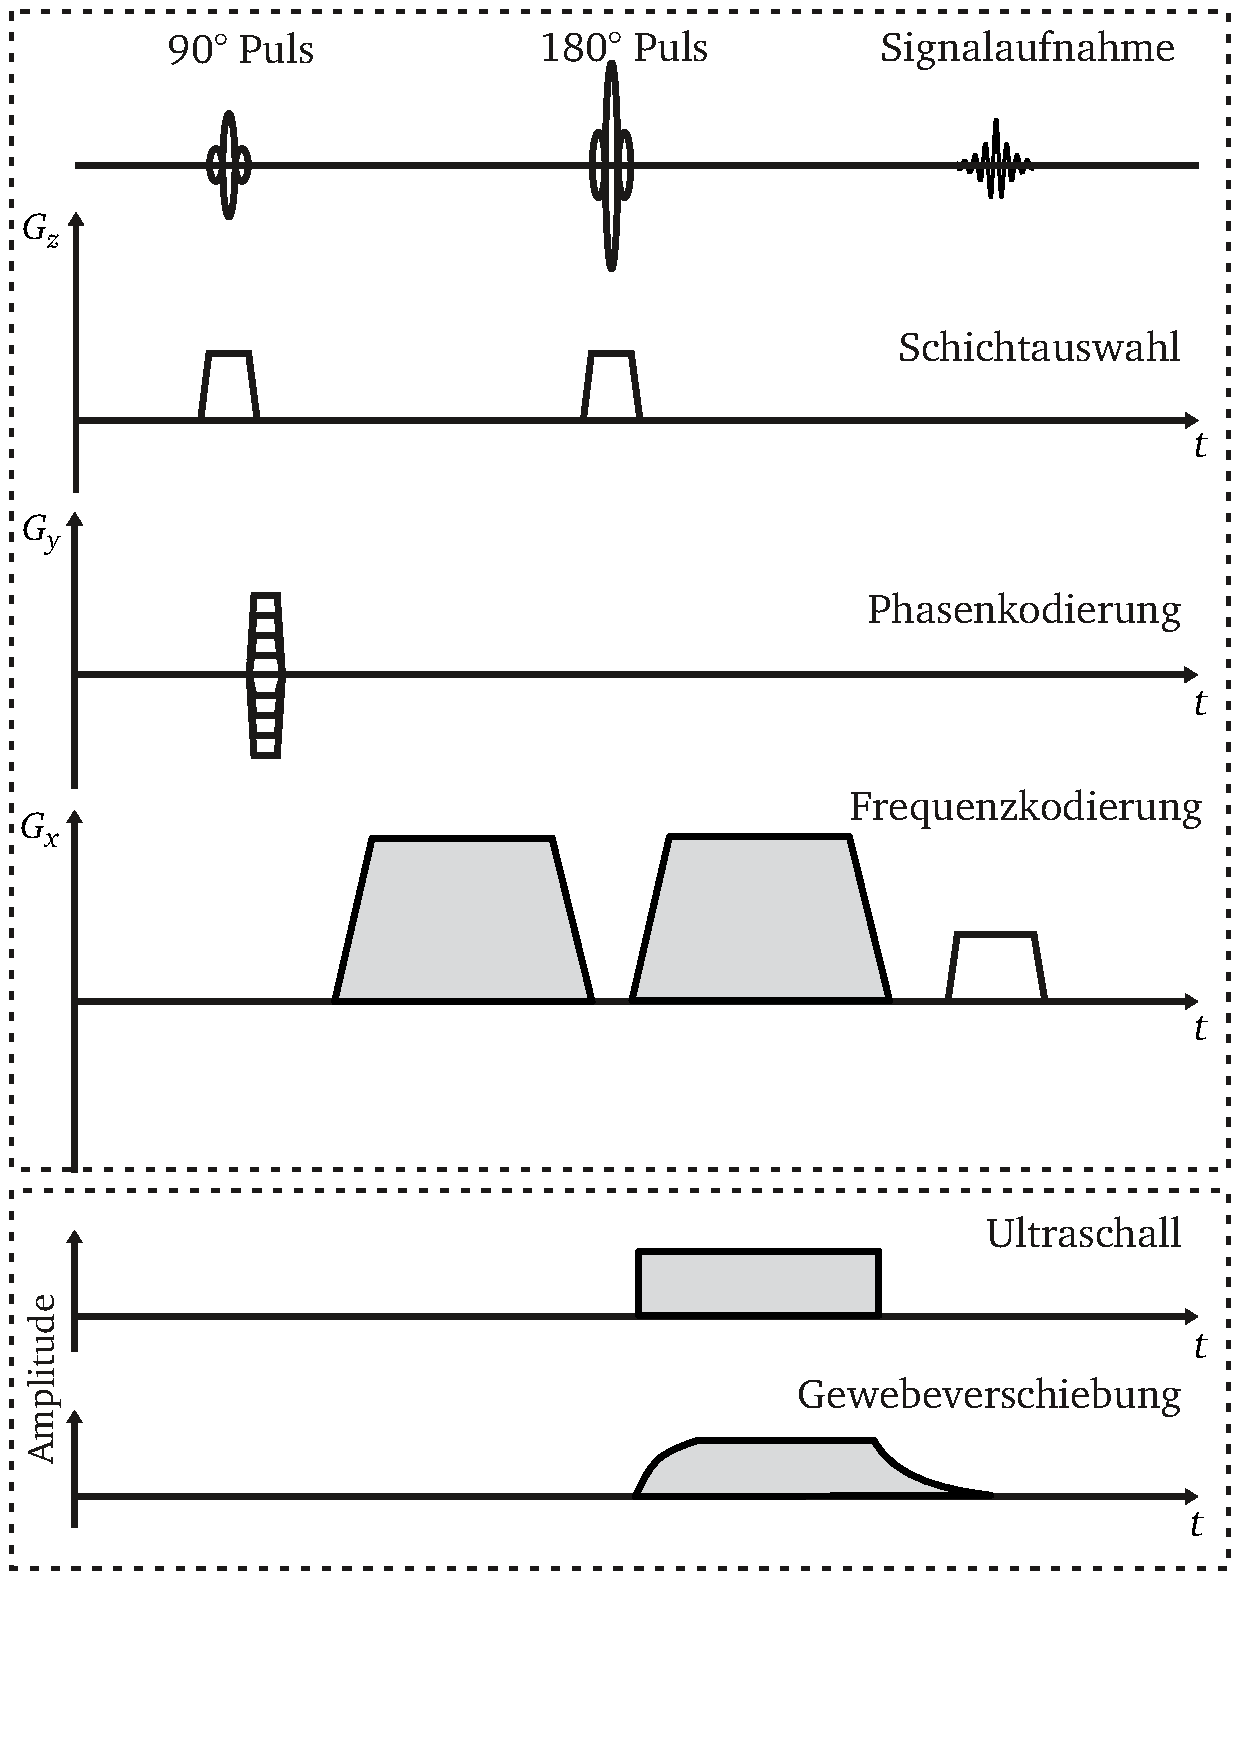
\includegraphics[width=.7\textwidth]{Abbildungen/sediffmono.pdf}
    \caption{%
        Bewegungssensitive MRT-Sequenz mit Gradienten zur Ortsauflösung. Durch den Ultraschall wird eine Gewebeverschiebung verursacht, die durch die grauen Gradienten $G_x$ sichtbar gemacht werden kann.
    }
    \label{fig:bew-sens-sequenz}
\end{figure}

\subsection{Bewegungssensitive Sequenzen}

Um eine Gewebeverschiebung im MRT-Bild sichtbar machen zu können, werden symmetrisch um den $\piup$-Puls zwei identische Gradienten $G_x$ der Dauer $T_G$ geschaltet (Abbildung~\ref{fig:bew-sens-sequenz}, grau). Der erste Gradient sorgt dabei für eine Phasenverschiebung abhängig von der $x$-Koordinate. Der $\piup$-Puls spiegelt nun die Magnetisierung. Findet keine Bewegung statt, macht der zweite Gradient die Phasenverschiebung daher Rückgängig. Ist das Gewebe allerdings bewegt worden, findet keine vollständige Rephasierung statt. Die Phasendifferenz ist dann konstant und kann mit
\[
    \Deltaup \phi = \gamma \cdot G_x T_G \Deltaup x
\]
in eine Verschiebung umgerechnet werden.


\section{Versuchsvorrichtung}

\begin{figure}[htbp]
    \centering
    \resizebox{\textwidth}{!}{% Tikzpicture Verschiebevorrichtung
    \begin{tikzpicture}
        % PC
        \draw (0,0) rectangle (1,1);
        \draw (-.2,-.2) rectangle (1.2,1.2);
        \draw (-.2,-.2) -- (-.4,-.4) -- (1.4,-.4) -- (1.2,-.2);
        \node at (.5,.5) {PC};

        % Kabel
        \draw[out=0, in=180]
            (1.2,.4) to (3,-.55)
            (1.2,.5) to (3,.45)
            (1.2,.6) to (3.,1.45);

        % Steuerbox mit Schrittmotoren
        \draw (3.,-1.1) rectangle (7,2);
        \foreach \y in {-1.0,0,1}
        \draw (3,\y) rectangle node{1} (4,\y+.9);

        % Kolben
        % Kolben 1
        \draw (4, -.7) rectangle (5.5,-.4);
        \draw[ultra thick] (4,-.55) -- (4.5,-.55);
        \draw (4.5,-.7) rectangle (4.6,-.4);

        % Kolben 2
        \draw (4, .3) rectangle (6.8,.6);
        \draw[ultra thick] (4,.45) -- (4.5,.45);
        \draw (4.5,.3) rectangle (4.6,.6);

        % Kolben 3
        \draw (4, 1.3) rectangle (5.,1.6);
        \draw[ultra thick] (4,1.45) -- (4.5,1.45);
        \draw (4.5,1.3) rectangle (4.6,1.6);

        % Verschiebevorrichtung
        \draw (8.7,-.2) rectangle (11.8,1.1);

        % Kolben 2
        \draw (8.8,.3) rectangle (11.6,.6);
        \draw[ultra thick] (9.4,.45) -- (12,.45);
        \draw (9.3,.3) rectangle (9.4,.6);

        % Kolben 1
        \draw (12,1.2) rectangle (12.3,-.3);
        \draw[ultra thick] (12.15,.6) -- (12.15,-.7);
        \draw (12,.7) rectangle (12.3,.6);

        % Kolben 3
        \draw (12.4,.9) rectangle (13.4,1.2);
        \draw[ultra thick] (13.0,1.05) -- (13.8,1.05);
        \draw (12.9,.9) rectangle (13.0,1.2);

        % Verbindung Kolben 1, 3 Emitter und Spiegel
        \draw (12.1,-.7) -- (12.4,-.7) -- (12.4,1.2);
        \draw (12.4,.5) -- (12.5,.5) coordinate (a) ;
        \draw (12.4,.8) --  (12.5,.8) coordinate (b);
        \draw[bend left] (b) to (a);
        \draw  ($(b)!.5!(a)$) -- (12.7,0) node[below]{4} ;
        \draw (13.8, 1.2) -- (13.8, 0.9);
        \draw (13.7,.9) rectangle coordinate (spiegel) (13.9,.4);
        \draw (spiegel) -- (13.5,0) node[below]{5};

        % Schläuche mit Steckverbindung und Kupplungen

        \draw[double] (5.4,-.4) to [out=90, in=-90] (6.9,.4) to [out=90, in=-90] (6.6,2) to [out=90, in=180] (7.6,2.6) -- (8.,2.6);
        \draw[ultra thick] (7.6,2.6) -- coordinate (S1)  (7.8,2.6) ;
        \draw (8.,2.5) rectangle coordinate (K1) (8.3,2.7);
        \draw[double] (8.3,2.6) -- (8.55,2.6);
        \draw[double] (8.65,2.6) to [out=0, in=90] (12.15,1.2);

        \draw[double] (6.6,.6) to [out=90, in=-90] (6.5,2) to [out=90, in=180] (7.6,2.3) -- (8.,2.3);
        \draw[ultra thick] (7.6,2.3) --  coordinate (S2) (7.8,2.3) ;
        \draw (8.,2.4) rectangle coordinate (K2) (8.3,2.2);
        \draw[double] (8.3,2.3) -- (8.51,2.3);
        \draw[double] (8.61,2.3) to [out=0, in=90] (9,.6);
        
        \draw[double] (4.9,1.6) to [out=90, in=-90] (6.4,2) to [out=90, in=180] (7.6,2.9) -- (8.,2.9);
        \draw[ultra thick] (7.6,2.9) -- coordinate (S3) (7.8,2.9);
        \draw (8.,2.8) rectangle coordinate (K3) (8.3,3.0);
        \draw[double] (8.3,2.9) -- (8.59,2.9);
        \draw[double] (8.69,2.9) to [out=0, in=90] (12.6,1.2);

        \draw (8.5,2.2) -- (8.6,3.0);
        \draw (8.6,2.2) -- (8.7,3.0);

        \node (S) at (7.5,3.8) {2};
        \foreach \y in {(S1), (S2), (S3)}
            \draw (S) -- \y;

        \node (K) at (8.3,3.8) {3};
        \foreach \y in {(K1), (K2), (K3)}
            \draw (K) -- \y;

        % Druckausgleich

            \draw (13.,-2) rectangle node {6} (13.75,-1);

            \draw[double] (12,-.2) to [out=180, in=180] (13,-1.3);
            \draw[double] (11.5,.3) to [out=-90, in=180] (13,-1.4); 
            \draw[double](13.3,.9) to [out=-90, in=180] (13,-1.2);

        % Beschriftung
        \node at (0,4) {\parbox{4.5cm}{
                1: Schrittmotor \\
                2: Steckverbindung \\
                3: Kupplung, tropffrei \\
                4: Ultraschallemitter \\
                5: Spiegel \\
                6: Druckausgleichsbehälter
            }
        };
    \end{tikzpicture}
}
    \caption{%
        Verschiebevorrichtung
    }
    \label{fig:aufbau_total}
\end{figure}


\chapter{Durchführung}

\section{Verbesserung der Versuchsvorrichtung}

An der vorhandenen Versuchsvorrichtung bestanden zu Anfang meiner Arbeit einige
Probleme die es zu verbessern galt. Zum Einen ließen sich die Kolben nach
einiger Zeit des Stehens nur sehr schwergängig in ihren Zylindern bewegen.
Damit die Schrittmotoren nicht überfordert würde musste man diese vor der
Benutzung per Hand lockern. Zum Anderen trat Luft bei Benutzung der Apperatur
in das System ein, wodurch nach einigem Fahren die Eichung der Verschiebung
nicht mehr stimmte.  

\subsection{Problem: Dichtungsringe}

Zum abdichten waren auf den Kolben zwei O-Ringe in jeweils eine Nut
eingelassen. Diese Nuten waren nur minimal breiter als die Schnurstärke der
Ringe. Befand sich der Kolben nun im Zylinder wurden die Ringe stark verformt
(Abbildung \ref{fig:nut_schmal}). Die dadurch entstehende breite Auflagefläche
und starke Rückstellkraft sorgt für hohe Reibung. Ist die Nut breiter kann sich
der Ring besser verformen (Abbildung \ref{fig:nut_breit}). Wird zudem noch die
Nut tiefer gestochen, verringert sich die Verformung und damit die
Auflagefläche und Rückstellkraft deutlich. Die Reibung schrumpft.

Da wir bei unserem Versuchsaufbau mit geringen Drücken zu tun haben, reicht
zudem eine Abdichtung mit nur einem O-Ring pro Kolben, statt der vorher
verwendeten zwei.

\begin{figure}[htbp]
\begin{minipage}[htbp]{.45\textwidth}
    \centering
    % Tikzpicture Dichtungsring in schmaler Nut
        \begin{tikzpicture}
            \draw[gray, fill=gray] (.5,0) -- (2,0) -- (2,-2.5) -- (5,-2.5) -- (5,0) -- (6.5,0) -- (6.5,-3.5) -- (.5,-3.5) -- (.5,0);
            \draw (.5,0) -- (2,0) -- (2,-2.5) -- (5,-2.5) -- (5,0) -- (6.5,0);
            \draw (3.5,-1.05) circle (1.43);
            \draw[dashed] (.5,.07) -- (6.5,.07) -- (6.5,.27) -- (.5,.27) -- (.5,.07);
            \foreach \x in {2.7, 3.5, 4.3} \draw[ultra thick, ->, dashed] (\x,-.8) -- (\x,0.05);
            \draw[dashed] (2.7,.05) 
            -- (4.3,.05) 
            arc (90:0:.68) 
            -- (4.98,-1.8) 
            arc (0:-90:.68)
            -- (2.7,-2.48)
            arc (-90:-180:.68)
            -- (2.02,-.63)
            arc (-180:-270:.68);

            % Beschriftungen
            \draw (1.,.17) -- (1.5,.7) node[above] {Zylinderwand};
            \node at (3.5,-2.9)  {Kolben mit Nut};
            \node at (3.5,-1.7) {O-Ring};
        \end{tikzpicture}

    \caption{%
        Querschnitt durch O-Ring in Nut. Breite Auflagefläche des O-Rings bei zu schmaler Nut.
    }
    \label{fig:nut_schmal}
\end{minipage}
\hfill
\begin{minipage}[htbp]{.45\textwidth}
    \centering
    % Tikzpicture für Dichtungsring in breiter Nut
        \begin{tikzpicture}
            \draw[gray, fill=gray] (1,0) -- (2,0) -- (2,-2.5) -- (6,-2.5) -- (6,0) -- (7,0) -- (7,-3.5) -- (1, -3.5) -- (1,0) ;
            \draw (1,0) -- (2,0) -- (2,-2.5) -- (6,-2.5) -- (6,0) -- (7,0) ;
            \draw (4,-1.05) circle (1.43);
            \draw[dashed] (1,0.07) -- (7,0.07) -- (7,.27) -- (1,.27) -- (1,.07) ;
            \foreach \x in {3.6, 4.4} \draw[ultra thick, ->, dashed] (\x,-.8) -- (\x,0.05);
            \draw[dashed] (3.6,.05) 
            -- (4.4,.05) 
            arc (90:-90:1.26) 
            -- (3.6,-2.48)
            arc (-90:-270:1.26);

            % Beschriftungen

            \draw (1.5,.17) -- (2.0,.7) node[above] {Zylinderwand};
            \node at (4.0,-2.9)  {Kolben mit Nut};
            \node at (4.0,-1.7) {O-Ring};
        \end{tikzpicture}

    \caption{%
        Querschnitt durch O-Ring in Nut. Kleine Auflagefläche wenn die Nut deutlich breiter ist als der O-Ring.
    }
    \label{fig:nut_breit}
\end{minipage}
\end{figure}

Ein weiterer Faktor ist die Wahl des Schmiermittels. Bisher wurde das
Silikonbasierte \emph{High Vacuum Grease}\footnote{Hersteller} verwendet. Ich
hab mich für eine Verwendung von \emph{Hochleistungs
\textsc{PTFE}-Spray}\footnote{Hersteller} entschieden, da dieses auch nach
längerem Stehen unter Druck gute Laufeigenschaften hat.


\subsection{Problem: Kupplung}

\subsection{Kalibrierung}

\section{Verbesserung der Versuchsvorrichtung}

\subsection{Problem: Bildstörungen}

\chapter{Ergebnis/Ausblick}

\end{document}

%vim: tw=79
